\section{Micrografías SEM de probetas FBPO}
\label{anx:SEM_imagenes}

En esta sección se presentan las micrografías SEM de las probetas FBPO.

\begin{figure}[h!]
    \centering
    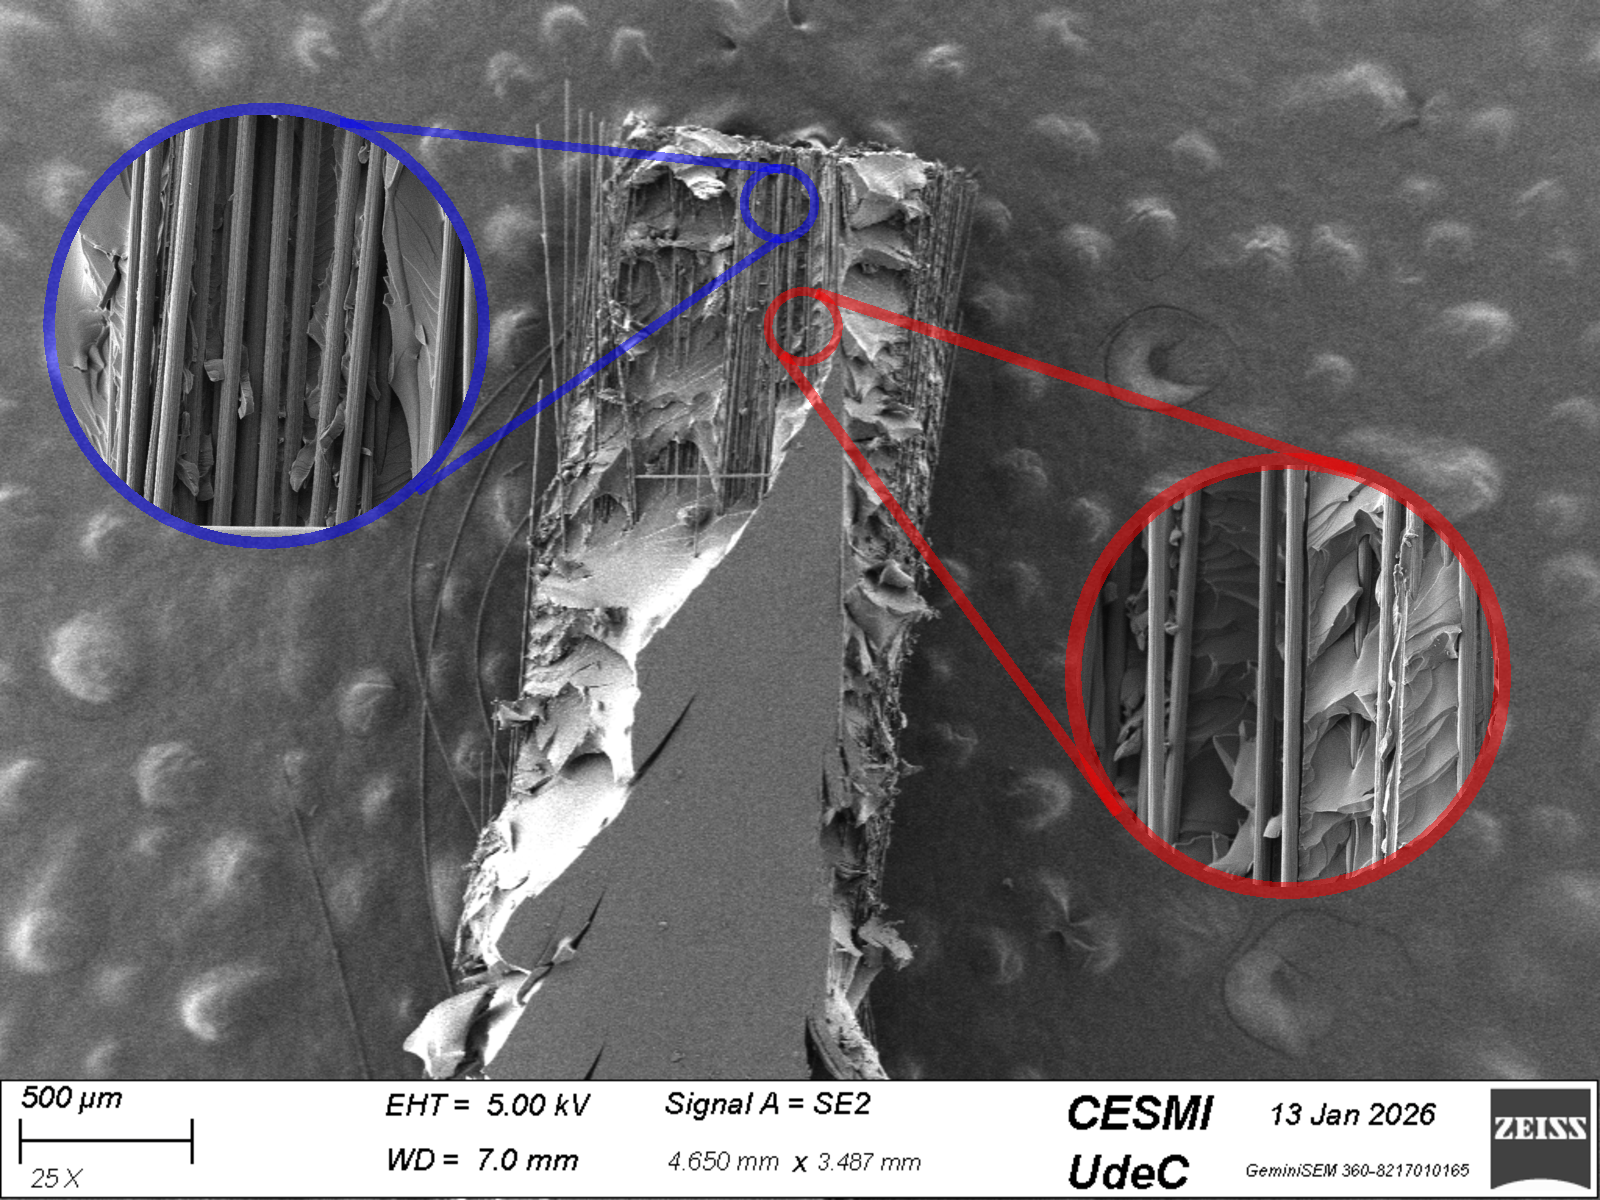
\includegraphics[width=0.75\textwidth]{SEM_MEPOX_color.pdf}
    \captionsetup{justification=centering, singlelinecheck=false}
    \caption{Micrografías SEM de las probetas FBPO, sistema MEPOX-HTA.}
    \label{fig:sem_mepox_color}
\end{figure}

\begin{figure}[h!]
    \centering
    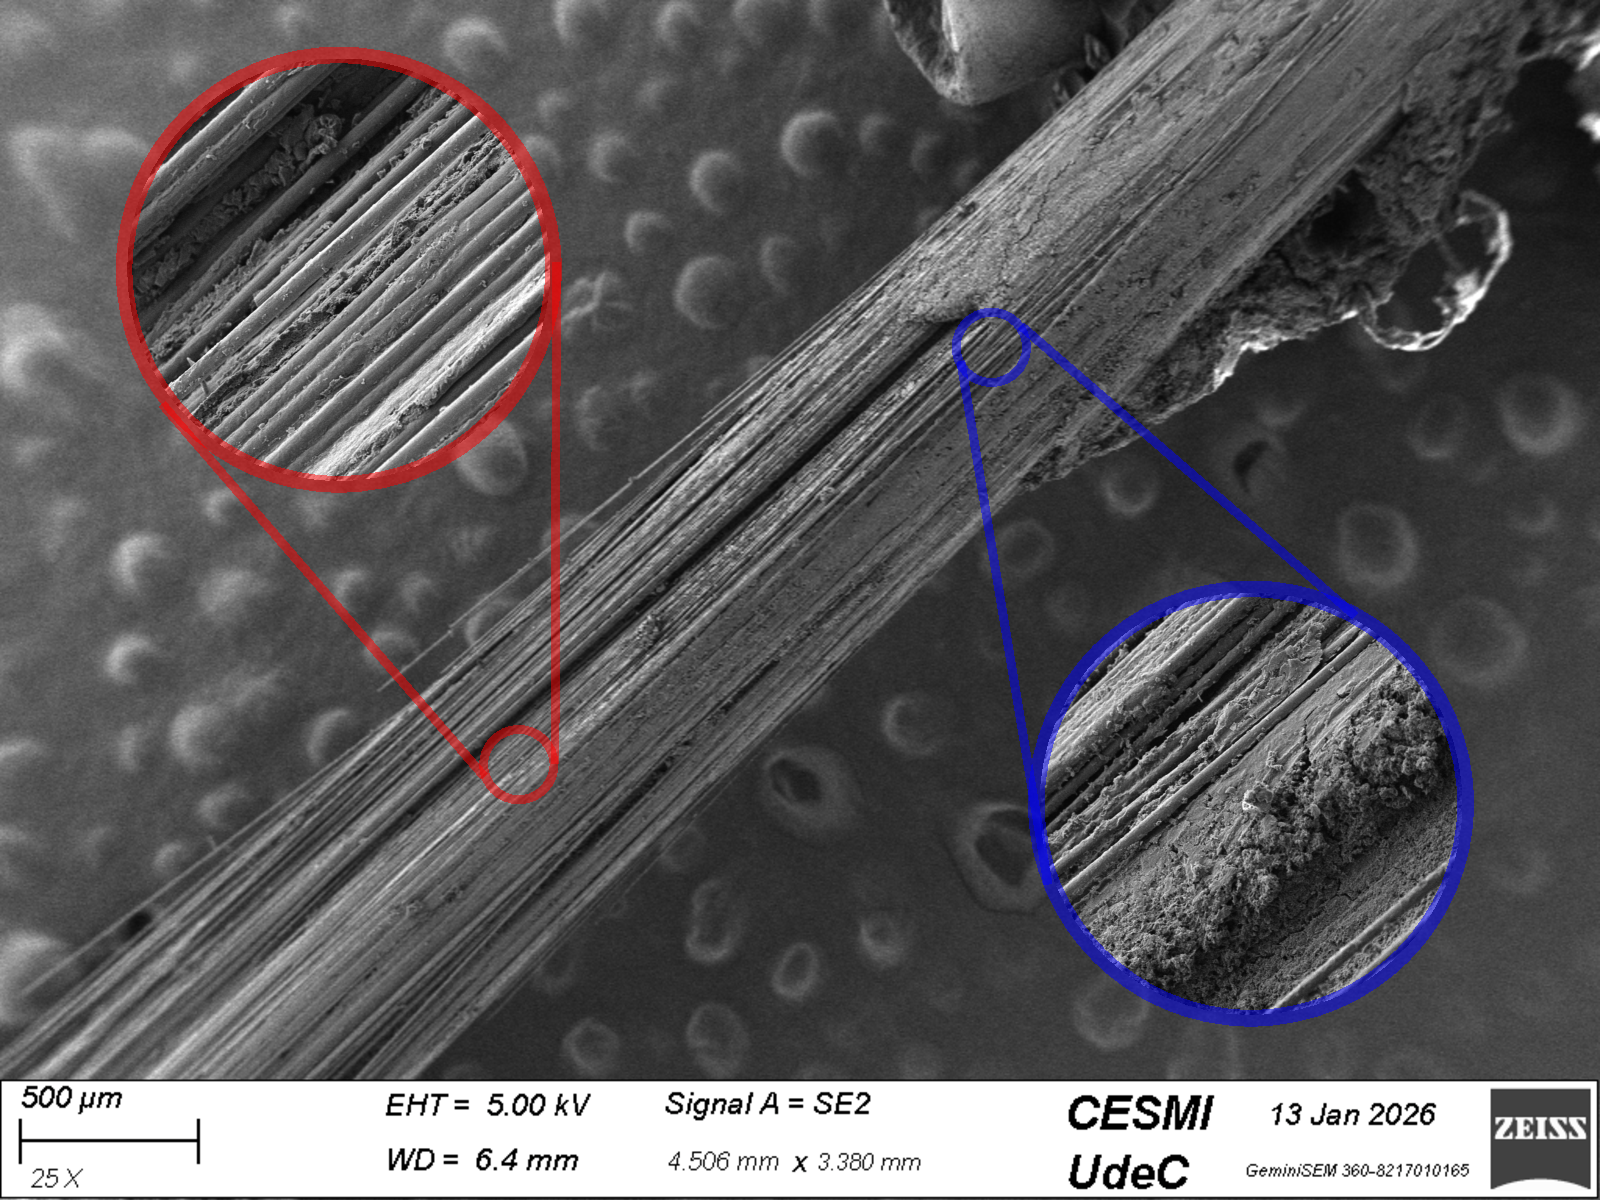
\includegraphics[width=0.75\textwidth]{SEM_EPO_color.pdf}
    \captionsetup{justification=centering, singlelinecheck=false}
    \caption{Micrografías SEM de las probetas FBPO, sistema EPO-HTA.}
    \label{fig:sem_epo_color}
\end{figure}

\begin{figure}[h!]
    \centering
    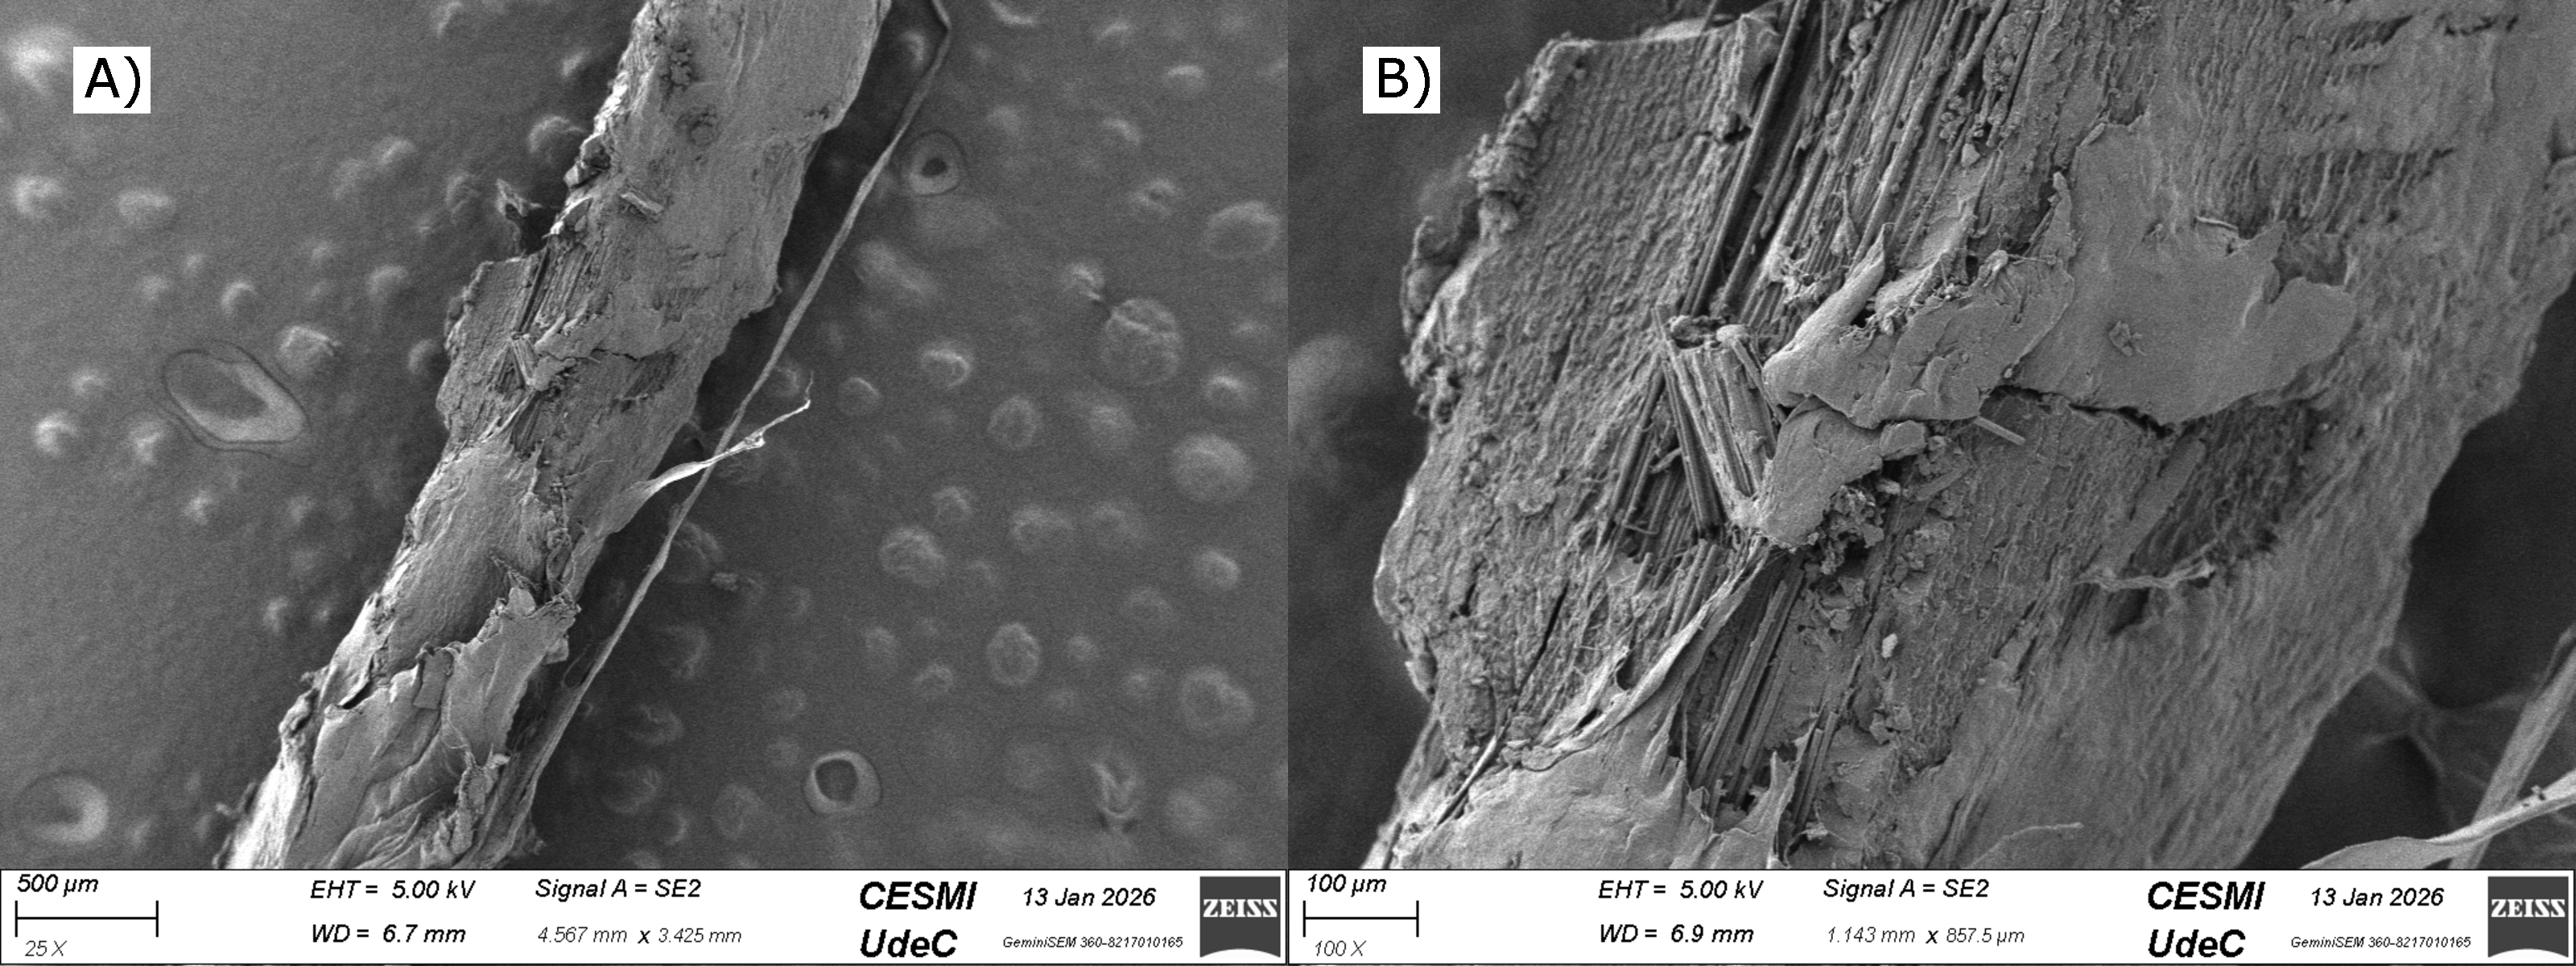
\includegraphics[width=0.9\textwidth]{SEM_TEFLON.pdf}
    \captionsetup{justification=centering, singlelinecheck=false}
    \caption{Micrografías SEM de las probetas FBPO, con restos de PTFE en la zona de la matriz.
    A) Probeta con restos de PTFE en la zona de la interfase, B) Acercamiento a varios filamentos.}
    \label{fig:sem_teflon}
\end{figure}

\begin{figure}[h!]
    \centering
    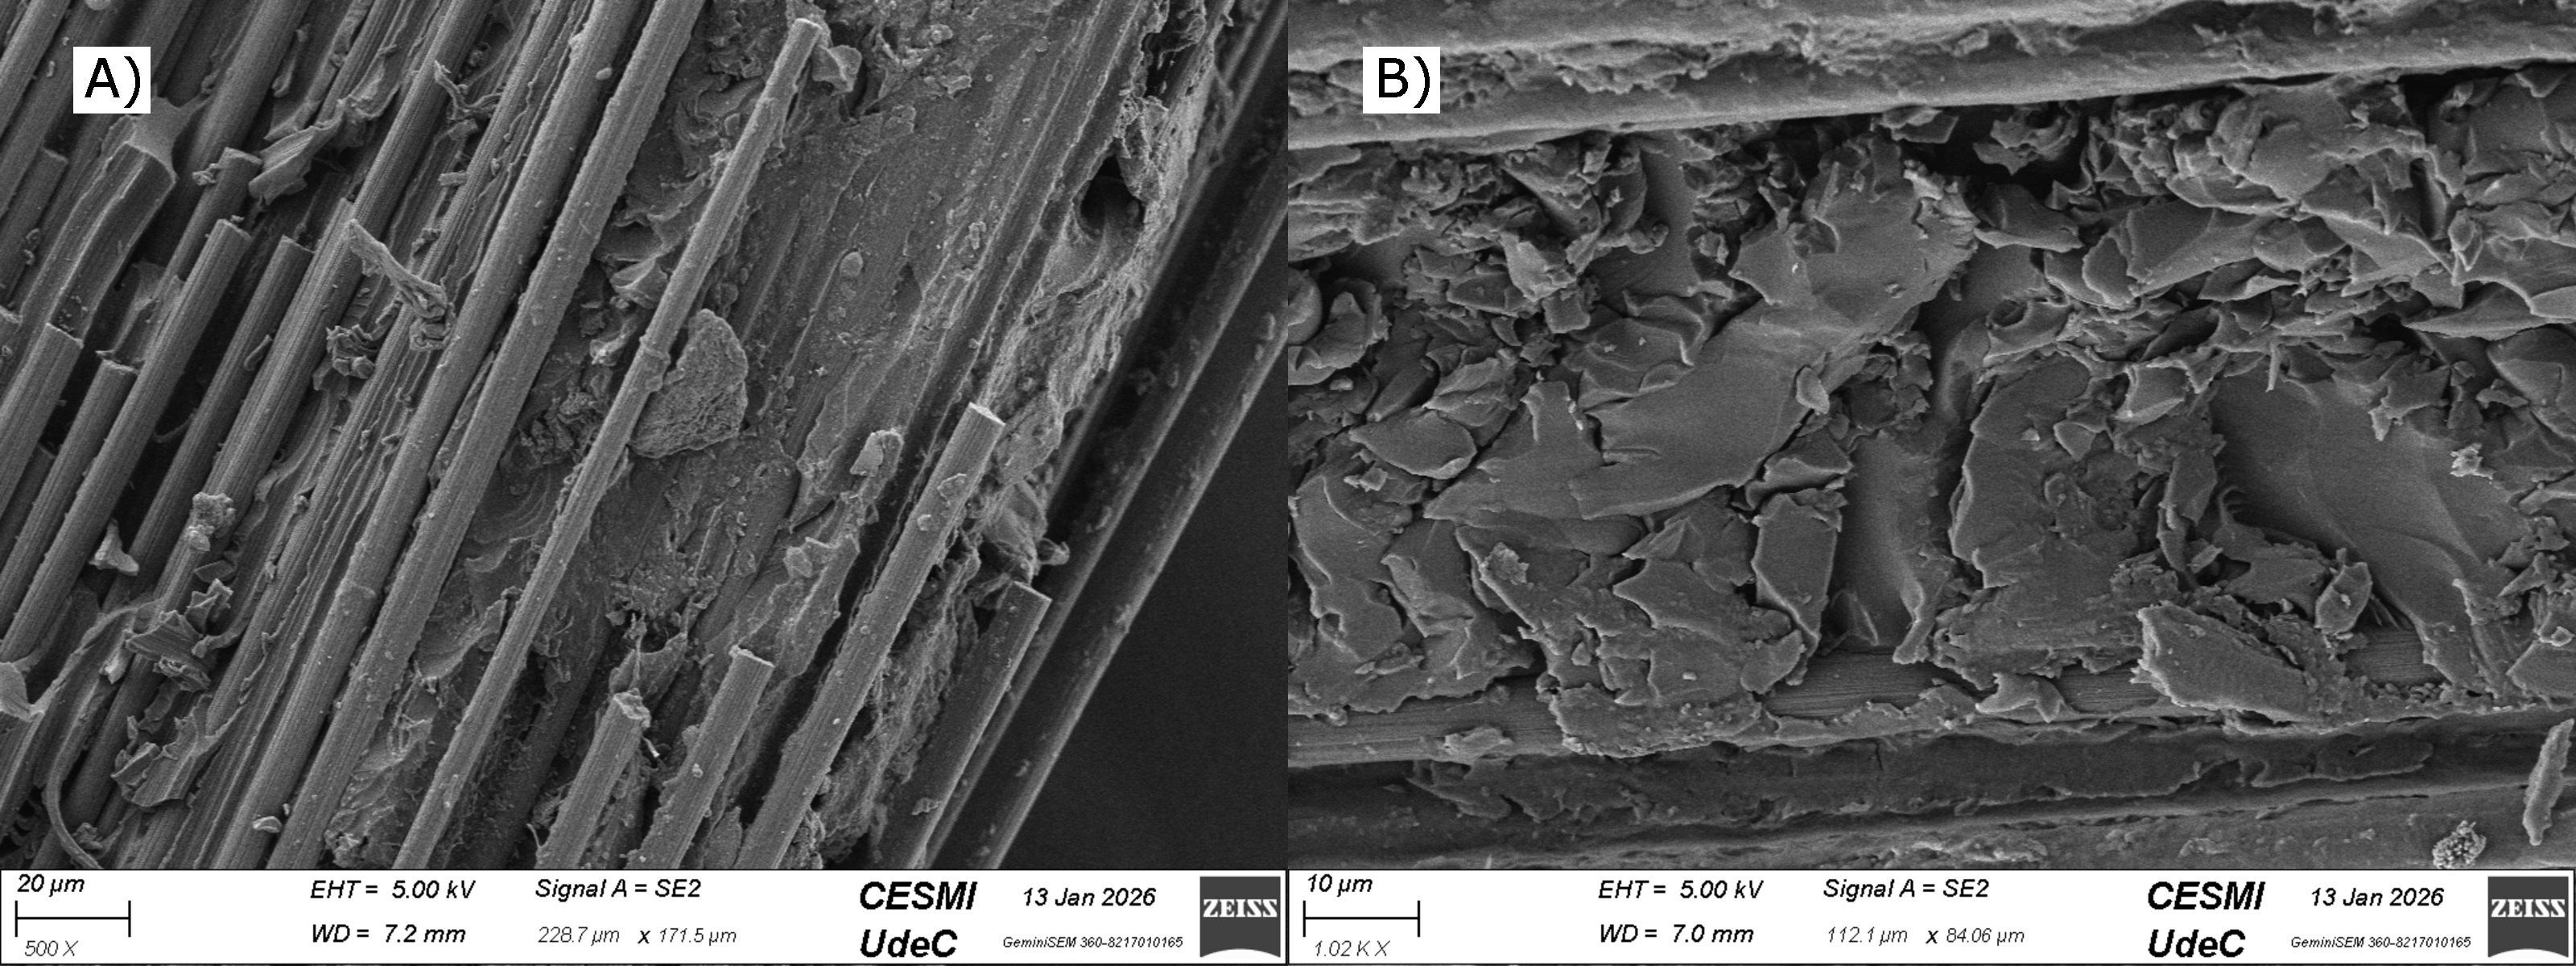
\includegraphics[width=0.9\textwidth]{SEM_comparativa.pdf}
    \captionsetup{justification=centering, singlelinecheck=false}
    \caption{Micrografías SEM de las probetas FBPO, comparativa entre MEPOX (A) y EPO (B).}
    \label{fig:sem_comparativa}
\end{figure}